意見間距離の平均値と人数$N$との間の関係

実際にはこれまで考えたクラスターから1つの意見が代表して選ばれ、時間が1進むごとに、そこから一番近い位置にあるクラスターからまた1つ意見が選ばれていくような過程を考えているので、選ばれた意見から構成されるネットワークは、単純に一本の線状に乗るようなネットワークを構成する。したがって、一般的なネットワークの特徴量ではなく、意見空間という位置の情報を含めたものであることを利用して、1つの意見ごとの平均距離(ネットワーク科学でいうところのノード間距離とは異なるものであることに注意)を測り、これが会議の参加人数とどのような関係であるかを見ていくことにする。

以下のグラフは、一人あたりの意見の数$S=20$、意見のクラスタ化閾値$r=0.07$としたときの、参加者の人数$N$と選ばれた意見間の距離の平均値$l$の関係を示したものである。
\begin{figure}[H]
    \begin{center}
        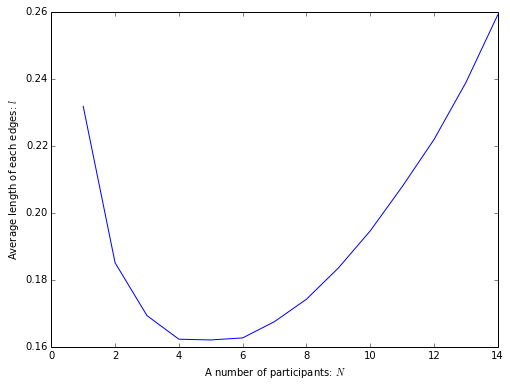
\includegraphics[width=12.5cm]{../img/N_l.png}
        \caption{ステップ間距離の平均値と$N$の間の関係}
        \label{fig:f24}
    \end{center}
\end{figure}
このグラフを見て分かるように、$l$は$N$の関数として見たとき下に凸な関数となっており、この$l$と会議の質との間に負の相関があるとすれば、この$l$は人数と会議の質の間の関係を示す指標となりうることが分かる。

さて、このようなグラフとなるのは、先程まで考えたように人の数が増えると意見の密度が大きくなり、同じ$r$でも、クラスターの融合が進むので、結果的にクラスター間の距離は離れることとなるということと、意見の密度が小さいときには、クラスターは形成されにくいが、逆に意見間の距離は広がるために、選ばれた意見間の距離も大きくなることになる。

また、今回は横軸の変数として人の数$N$を変更させていったが、参加者の発言頻度が会議の質との関係がないと仮定した場合には、一人あたりの意見の数$S$を変えた場合と完全に等価になる。すなわち、横軸に$M=S\times N$としてグラフを描くこともできる。

はじめに考えたように、このように意見空間において意見のクラスター化を行うということは、近すぎる内容の意見は人は発言しないということを意味しており、この結果、参加する人数が大きいほど、それぞれの人がいいそうなことが予想されるので、当人としては当然の流れとして、一つ前の意見から離れた意見を選ぶことが許されることになる。しかし、あまりに意見間の距離が大きくなると、参加している人の考えるつながりとは必ずしも一致しないので、そこに意見の飛躍が生じることによって「わからない意見」が増えることになる。一方で人の数が少なく、それぞれの意見の間に差が生じている時には、そもそも意見の間の差が大きいために、意見同士はつながりが小さくなる。


